\section{Geometrie}
\subsection{Planimetrie}
\subsubsection{Strahlensätze}
%TODO picture
\paragraph{1.}
\begin{align*}
    \overline{SA_1} : \overline{SB_1} = \overline{A_1A_2} : \overline{B_1B_2} \\
    \overline{SA_1} : \overline{SA_1} = \overline{SB_1} : \overline{SB_2} \\
\end{align*}
Entsprechende Abschnitte auf den Strahlen stehen im gleichen Verhältnis

\paragraph{2.}
\begin{align*}
    \overline{CB} : \overline{C_1B_1}: \overline{C_2B_2}    &= \overline{SC} : \overline{SC_1} : \overline{SC_2}  \\
                                                            &= \overline{SB} : \overline{SB_1} : \overline{SB_2}  \\
\end{align*}
\begin{align*}
    \overline{AB} : \overline{A_1B_1}: \overline{A_2B_2}    &= \overline{SA} : \overline{SA_1} : \overline{SA_2}  \\
                                                            &= \overline{SB} : \overline{SB_1} : \overline{SB_2}  \\
\end{align*}
Entsprechende Abschnitte auf den Parallelen stehen im gleichen Verhältnis wie die zugehörigen, vom Scheitel aus zu messenden Abschnitte auf den Strahlen.

\paragraph{3.}
\begin{align*}
    \overline{AB} : \overline{BC} = \overline{A_1B_1} : \overline{B_1C_1} = \overline{A_2B_2} : \overline{B_2C_2} \\
\end{align*}
Entsprechende Abschnitte auf den Parallelen stehen im gleichen Verhältnis.

\subsubsection{Satz des Pythagoras}
%TODO picture

\begin{figure}[htb]
\begin{center}
%	\includegraphics[height=1in,width=1in,angle=-90]{./08_Geometrie/pythagoras.standalone}
	\includegraphics[height=1in,width=1in,angle=-90]{pythagoras.standalone.eps}
\caption{This is a figure.}
\end{center}
\end{figure}

%\begin{figure}
%    \centering
%    \subfloat{
%	\includegraphics[height=2in,width=2in,angle=-90]{sections/08_Geometrie/pythagoras.standalone.pdf}
%   }\hfill
%   \subfloat{
%      \begin{minipage}[t]{120mm}
%   	$A = \frac{d^2 \cdot \pi}{4}$ \\
%	$U = d \cdot \pi  $
%      \end{minipage}
%    }
%  \caption{Abbildungsname}
%  \label{fig:decision-tree}
%\end{figure}


\begin{align*}
    a^2+b^2=c^2
\end{align*}

\subsubsection{Höhensatz des Euklid}
%TODO picture
\begin{align*}
    h^2=p \cdot q
\end{align*}



\subsubsection{Kathetensatz}
%TODO picture
\begin{align*}
    a^2=c \cdot p \\
    b^2=c \cdot q \\
\end{align*}

\subsubsection{Trapez}
%TODO picture
\begin{align*}
    A &= \frac{a+b}{2} \cdot h = m \cdot h \\
    m &= \frac{a+b}{2}
\end{align*}

\subsubsection{Kreis}
%TODO picture
\begin{align*}
    A &= \frac{d^2 \cdot \pi}{4} \\
    U &= d \cdot \pi \\
\end{align*}

\subsubsection{Kreisausschnitt}
%TODO picture
\begin{align*}
    A &= \frac{d^2 \cdot \pi}{4} \cdot \frac{\alpha^\circ}{360^\circ} = \frac{b \cdot r}{2} \\
    b &= \frac{d \cdot \pi \cdot \alpha^\circ }{ 360^\circ} \\
\end{align*}

\subsubsection{Ellipse}
%TODO picture
\begin{align*}
    A &= \frac{D \cdot d \cdot \pi}{4} = a \cdot b \cdot \pi \\
    U &\approx \frac{D+d}{2} \cdot \pi \\
\end{align*}


\subsection{Stereometrie}
\paragraph{Gerade Körper}
\begin{align*}
    V = A \cdot h
\end{align*}

\paragraph{Spitze Körper}
\begin{align*}
    V = \frac{1}{3} \cdot A \cdot h
\end{align*}

\paragraph{Stumpfe Körper}
\begin{align*}
    V = \frac{1}{3} \cdot h ( A_1 + \sqrt{A_1 \cdot A_2} + A_2)
\end{align*}

\paragraph{Kugel}
\begin{align*}
    V &= \frac{4}{3} \cdot \pi \cdot r^3 \\
    O &= 4 \cdot \pi \cdot r^2 \\
\end{align*}

\subsection{Trigonometrie}
\subsubsection{Winkelfunktionen im rechtwinklichen Dreieck}
%TODO picture
\begin{align*}
    \sin \alpha &= \frac{\textrm{Gegenkathete}}{\textrm{Hypotenuse}}  &= \frac{a}{c} \\
    \cos \alpha &= \frac{\textrm{Ankathete}}{\textrm{Hypotenuse}}     &= \frac{b}{c} \\
    \tan \alpha &= \frac{\textrm{Gegenkathete}}{\textrm{Ankathete}}   &= \frac{a}{b} \\
    \cot \alpha &= \frac{\textrm{Ankathete}}{\textrm{Gegenkathete}}   & = \frac{b}{a} \\
\end{align*}

\paragraph{Trigonomische Beziehungen der Komplementwinkel}
\begin{align*}
    \sin \alpha &= \cos \beta  = \cos (90^\circ - \alpha) \\
    \cos \alpha &= \sin \beta  = \sin (90^\circ - \alpha) \\
    \tan \alpha &= \cot \beta  = \cot (90^\circ - \alpha) \\
    \cot \alpha &= \tan \beta  = \tan (90^\circ - \alpha) \\
\end{align*}


\subsubsection{Winkelfunktionen im spitz- und stumpfwinklichen Dreieck}


\paragraph{Sinussatz}
%TODO picture
\begin{align*}
    a : b : c = \sin \alpha : \sin \beta :\sin \gamma \\
    \frac{a}{\sin \alpha} = \frac{b}{\sin \beta} = \frac{c}{\sin \gamma}
\end{align*}

\paragraph{Kosinussatz}
%TODO picture
\begin{align*}
    a^2 = b^2 + c^2 -2bc \cos \alpha \\
    b^2 = c^2 + a^2 -2ca \cos \beta \\
    c^2 = a^2 + b^2 -2ab \cos \gamma \\
\end{align*}

\paragraph{Fläche eines Dreiecks}
\begin{align*}
    A = \frac{1}{2} ab \sin \gamma = \frac{1}{2} bc \sin \alpha = \frac{1}{2} ac \sin \beta
\end{align*}


\subsection{Geniometrie}
\subsubsection{Bogenmaß}
%TODO picture
\begin{align*}
    1  \textrm{ rad} = \frac{180^\circ}{\pi}        \\
    1 ^\circ = \frac{\pi}{180^\circ} \textrm{ rad}  \\
    x = \frac{b}{r} = \frac{\pi}{180^\circ} \cdot \alpha^\circ \\
\end{align*}

\subsubsection{Grundbeziehungen}
\begin{align*}
    \sin^2 \alpha + \cos^2 \alpha = 1 \textrm{ (Trigonomischer Pythagoras)} \\
    \tan \alpha = \frac{\sin \alpha}{\cos \alpha};
    \cot \alpha = \frac{\cos \alpha}{\sin \alpha};
    \tan \alpha \cdot \cot \alpha = 1
\end{align*}

\subsubsection{Winkelbeziehungen in den Quadranten}
\paragraph{$90^\circ \leq \alpha \leq 90^\circ$}
\begin{align*}
\sin \alpha &= \sin{(180^\circ-\alpha)} \\ 
\cos \alpha &= -\cos{(180^\circ-\alpha)} \\ 
\tan \alpha &= -\tan{(180^\circ-\alpha)} \\ 
\cot \alpha &= \cot{(180^\circ-\alpha)} \\ 
\end{align*}

\paragraph{$180^\circ \leq \alpha \leq 270^\circ$}
\begin{align*}
\sin \alpha &= -\sin{(\alpha-180^\circ)} \\ 
\cos \alpha &= -\cos{(\alpha-180^\circ)} \\ 
\tan \alpha &= \tan{(\alpha-180^\circ)} \\ 
\cot \alpha &= \cot{(\alpha-180^\circ)} \\ 
\end{align*}

\paragraph{$270^\circ \leq \alpha \leq 360^\circ$}
\begin{align*}
\sin \alpha &= -\sin{(360^\circ-\alpha)} \\ 
\cos \alpha &= \cos{(360^\circ-\alpha)} \\ 
\tan \alpha &= -\tan{(360^\circ-\alpha)} \\ 
\cot \alpha &= -\cot{(360^\circ-\alpha)} \\ 
\end{align*}


\subsubsection{Funktionen von Winkelsummen}

\begin{align*}
\sin{(\alpha \pm \beta)} &= \sin{\alpha} \cdot \cos{\beta} \pm \cos{\alpha}  \cdot \sin{\beta} \\
\cos{(\alpha \pm \beta)} &= \cos{\alpha} \cdot \cos{\beta} \pm \sin{\alpha}  \cdot \sin{\beta} \\
\tan{(\alpha \pm \beta)} &= \frac{\tan{\alpha} \pm \tan{\beta}}{1 \mp \tan{\alpha} \cdot \tan{\beta}} \\
\cot{(\alpha \pm \beta)} &= \frac{\cot{\alpha} \cdot \cot{\beta} \pm 1}{\cot{\beta} \pm \cot{\alpha}} \\
\end{align*}

\subsubsection{Summe von Winkelsummen}
\begin{align*}
\sin{\alpha} + \sin{\beta}  &= 2 \cdot \sin{\frac{\alpha+\beta}{2}} \cdot \cos{\frac{\alpha-\beta}{2}} \\
\sin{\alpha} - \sin{\beta}  &= 2 \cdot \cos{\frac{\alpha+\beta}{2}} \cdot \sin{\frac{\alpha-\beta}{2}} \\
\end{align*}

\subsubsection{Beziehung der doppelten Winkel}
\begin{align*}
\sin{ 2\alpha} &= 2 \sin{ \alpha} \cos{ \alpha} \\
\cos{ 2\alpha} &= \cos^2{ \alpha} - \sin^2{ \alpha} \\
\tan{ 2\alpha} &= \frac{2 \tan{\alpha}}{1-\tan^2{\alpha}} \\
\cot{ 2\alpha} &= \frac{\cot^2{\alpha}-1}{ 2 \cot{\alpha}}
\end{align*}



